\section{Introduction}
\label{sec:intro_new}

% --------------------------------------
% Mechanistic Interpretability outline
% --------------------------------------

% \av{Add: why this task , description of the different class of heads,
% Different part of the circuit and what they do (some are weird),
% High level presentation of the 4 criteria}

Current transformer-based language models (LMs) (\cite{Attention}, \cite{GPT3}) have demonstrated an impressive suite of capabilities, but largely remain black boxes. The interpretation of their inner computation is particularly challenging since they are composed of densely connected non-linear layers operating in a high-dimensional space. Previous attempts at understanding inner activations through correlation analysis (\cite{syntactic_Agreement_Mechanisms}, \cite{bert_nlp_pipeline}) will fail to generally understand \textit{how} models behave (\cite{antverg2021pitfalls}, \cite{attention_not_explanation}). Answering this causal question is the goal of interpretability, or transparency research.
% Despite the success of causal intervention \cite{meng2022locating} \cite{geiger2021causal} \cite{causal_syntactic_agreement} to locate relevant modules, these works doesn't provide a full picture of the mechanisms underlying the LM abilities.

%Extensive studies explored the origin of their linguistic abilities for syntactic processing \cite{syntactic_Agreement_Mechanisms}, sentiment analysis \cite{lstm_sentiment_neuron}, or general structure of their NLP  \cite{}. Nonetheless, these works relies on interpreting inner activation through correlation analysis. Such analysis of individual neurons or attention patterns, in the case of transformer-based model, has been shows to lead to misleading results \cite{} \cite{}. Even causal intervention can enable the localization of intermediate representation, such as facts \cite{rome}, linguistic entities 

Work in \textit{mechanistic interpretability} is a causal approach to understanding neural network behavior, that aims to reverse-engineer model computations into human-understandable components. This is particularly hard in the case of LMs, where models need to perform well at a variety of tasks in order to get low loss on their training data. Few existing works have been able to abstract the messy internals of LM models into higher-level components (`circuits'), except for contributions that study architectures chosen to be interpretable (\cite{elhage2021mathematical} does not include MLPs, for example). % \footnote{This work does not use MLPs due to difficulties understanding their intermediate activations}.

% Move this elsewhere!!!
%By understanding underlying mechanisms, we can better predict out-of-distribution behavior \citep{mu2020compositionalExplanations}, identify and fix model errors \citep{hernandez2021natural,vig2020investigating}, and understand emergent behavior \citep{meca_interp_grokking,barak2022hidden}. Some researchers have also argued that mechanistic interpretability is necessary for the safe deployment \citep{hendrycks2021unsolved} of advanced machine learning systems \citep{proposals,EvanTechTree,Hendrycks2022XRiskAF}.

We find a large circuit that implements a non-trivial linguistic task in GPT-2 small. Consider the sentence ``When Mary and John went to the store, John gave a bottle to Mary''. A capable language model should predict that the final token is ``Mary'', since this is the only appropriate name in the context to use - we call this capability Indirect Object Identification (IOI). Predicting `Mary' is not easily attributable to a single mechanism in a LM, but requires firstly locating the two names in the context and then discarding the name that has already appeared as the subject of the current clause. Our work explains this algorithmic behavior and therefore bridges the gap between current lower-level mechanistic techniques developed, and higher-level actual LM behaviors.

Our circuit contains 26 attention heads--1.1\% of the total number of (head, token position) pairs--that completes this task. While subsets of as few as 13 of these heads can achieve reasonable performance, we find that all 28 heads are necessary to fully account for the mechanisms used by GPT-2 small in this task. The heads fall into six major categories: \emph{name-mover}, \emph{subject-inhibition}, \emph{duplicate token}, \emph{negative name-mover}, \emph{induction} and \emph{previous-token}. A schematic of the circuit is shown in Figure~\ref{fig:the_circuit}.

\begin{figure*}
\centering
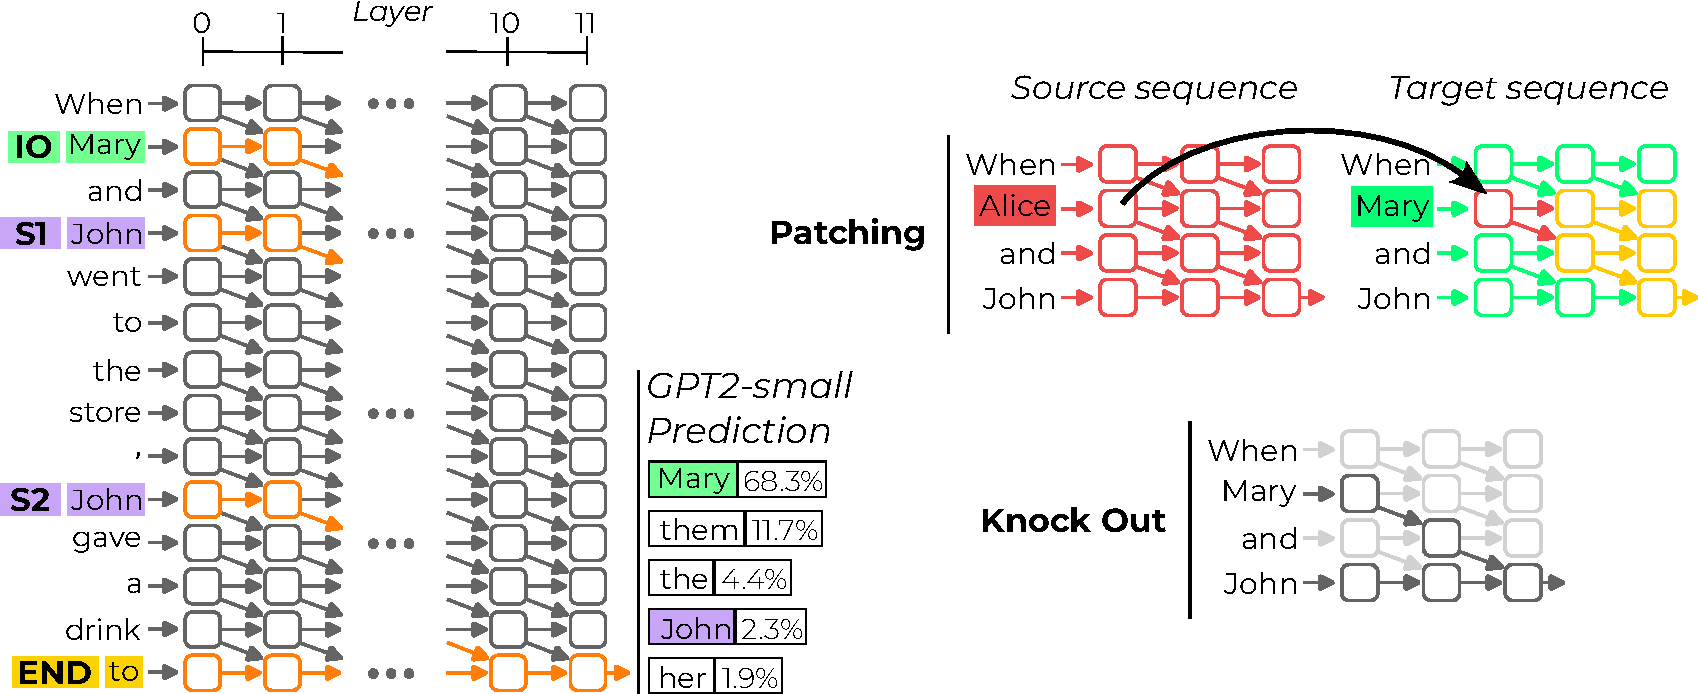
\includegraphics[width=0.9\textwidth]{figs/front_fig_v3.pdf}
\label{fig:directed_graph_figure}
\caption{Left: We isolated a \emph{circuit} (in orange) responsible for the flow of information connecting the indirect object 'Mary' to the next token prediction. The nodes are attention blocks and the edges represents the interactions between attention heads. Right: We discovered and validated this circuit using activation experiments, they include patching and knock out of attention heads. }
\end{figure*}

To verify that our circuit is correct, we formulate four criteria. The first is qualitative: our explanation is \textbf{legible} if the nodes in the circuit accurately correspond to human-understandable concepts. The other three quantitative criteria are that the model is \textbf{faithful} (the circuit is used to perform the task), \textbf{complete}  (the circuit contains all the nodes used to perform the task) and \textbf{minimal} (the circuit doesn't contain nodes irrelevant to the task).
% We empirically evaluate the completeness and minimality criteria using \emph{circuit extraction}: an exhaustive ablation method that isolates a circuit by ablating every node but the circuit. Our circuit passes these tests reasonably, though our understanding is still not complete \ac{I only think we can claim that we pass the tests `better' than other models, not that we objectively pass anything}.

% NEW EMPHASIS ON WHAT MATTERS
Thus, in summary, our main contributions are that we (i) identify a large circuit in GPT-2 small that performs IOI (Figure \ref{fig:the_circuit} and Section \ref{sec:methods}), (ii) provide a \textit{legible} interpretation of all the components of the circuit, based on causal interventions (Section \ref{sec:legibility}). We then finally (iii) evaluate our circuit against the standards of \textit{completeness} and \textit{minimality} through extensive experiments (Section \ref{sec:validation}).

%using known techniques such as causal interventions (activation patching) and original techniques such as `knockouts' (Section \ref{sec:knockouts}).

% END NEW EMPHASIS

% DELETING THE EMPHASIS ON THE CRITERIA
% Thus, in summary, our main contributions are that we (i) Identify a large circuit in GPT-2 small that performs IOI (Figure \ref{fig:the_circuit} and Section \ref{sec:methods}), (ii) present an empirical standard that can verify that any circuit explanation of model behavior both fully describes the behaviour and does not contain unnecessary detail (Section \ref{sec:criteria}). Finally we (iii) verify that that our circuit meets this standard, through extensive experiments (Sections \ref{sec:legibility} and \ref{sec:validation}), using known techniques such as causal interventions (activation patching) and original techniques such as `knockouts' (Section \ref{sec:knockouts}).
% FINISHED EMPHASIS DELETION